\section*{Aufgabe 3}

\subsection*{a)}
Sei $K_2$ definiert als $K_2=(Q_1 \cup \{ q_0, q_{acc}\} , \Sigma , \Gamma_2 , \delta_2 , Z_1, q_0, \{ q_{acc} \} )$.\\
 Mit $\Gamma_2 = \Gamma_1 \cup {E}$ und\\
Für $q \in Q_1$ ist $\delta_2 (q,a,z) = \delta_1 (q,a,z) $, \\
 $\delta_2 (q,\varepsilon ,E) = (q_{acc}, Z_1) $ \\
 $\delta_2 (q_0,\varepsilon ,Z_0) = (q_1, E Z_1) $\\
 Wie in :\\
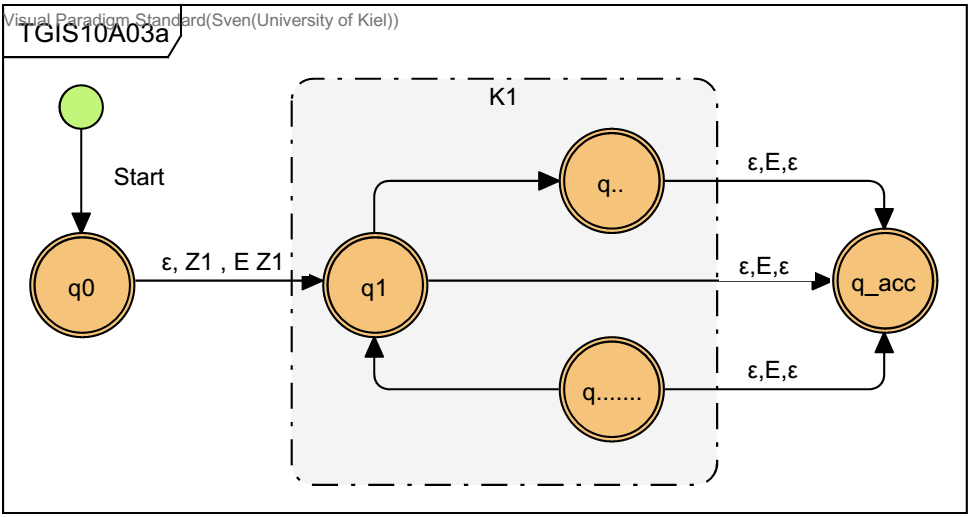
\includegraphics[width=\textwidth]{part/TGIS10A03a}\\
Idee:
Füge ein Unterstes Element in den Stack und übergehe in $K_1$ wenn ein Zustand keine Eingaben mehr hat und das oberste Element des Stacks das zuerst eingefügte ist gehe in  den akzeptierten zustand.



